\documentclass[numbers=noenddot,12pt,a4paper]{scrartcl}
\usepackage[greek,ngerman]{babel}
\usepackage[T1]{fontenc}
\usepackage[utf8]{inputenc}
\usepackage{fullpage}
\usepackage{libertine}
\usepackage{ziffer}
\usepackage{graphicx}
\usepackage{units}
\usepackage[infoshow]{tabularx}
\usepackage{amsmath}
\usepackage{amssymb}
\usepackage{wrapfig}
\usepackage{esint}
\usepackage{float}
\usepackage{wrapfig}
\usepackage[font=small]{caption}
\usepackage{subcaption}
\usepackage{lscape}
\usepackage{hyperref}

\renewcommand{\thefigure}{Abb. \arabic{figure}}

\captionsetup[wrapfigure]{name=}
\captionsetup[figure]{name=}
\newcommand{\degree}{^\circ}
\newcommand{\diff}{\textnormal{d}}
\newcommand{\tenpo}[1]{\cdot 10^{#1}}
\newcommand{\greek}[1]{\greektext#1\latintext}
\newcommand{\ix}[1]{_\text{#1}}
\newcommand{\imag}{\mathbf{i}}
\newcommand{\tilt}[1]{\textit{#1}}
\newcommand{\grad}[1]{\textit{grad}\left(#1\right)}
\newcommand{\divergenz}[1]{\textit{div}\left(#1\right)}
\newcommand{\euler}{\mathnormal{e}}
\newcommand{\fett}[1]{\textbf{#1}}

\title{Protokoll: Laser-Spektroskopie} %TODO Name des Versuchs eintragen
\author{Philipp Hacker} %TODO Protokollschreiber unterstreichen
\date{\today}

\begin{document}
%\setcounter{page}{2}
%\setcounter{section}{1}
\maketitle
\begin{center}
Betreuer: A.-P. Herrendorf\\ %TODO Name des Betreuers eintragen
Versuchsdatum: 03.12.2014\\ %TODO Datum des Versuchs eintragen
\begin{table}[h]
\centering
Note: %TODO Gute Note erhalten :)
\begin{tabularx}{1.5cm}{|X|}
\hline \\ \\
\hline
\end{tabularx}
\end{table}
\end{center}
\vspace*{\fill}
\tableofcontents
\vfill
\newpage
\section{Einleitung}
\section{Grundlagen}
\subsection{Festkörper-Laser}\label{subsec:fklaser}
\begin{wrapfigure}[15]{lo}{0.45\textwidth}
	\centering
	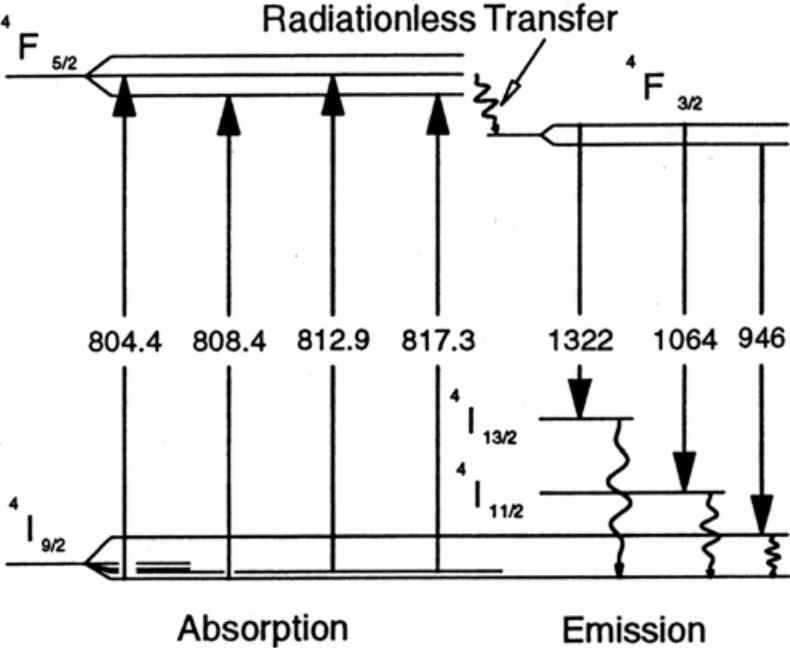
\includegraphics[width=0.425\textwidth]{uebergaenge.png}
	\caption{Schema der Übergänge in einem Vier-Niveau-Laser}\label{img:ueber}
\end{wrapfigure}
Diese Laser (\tilt{\textbf{L}ight \textbf{A}mplification} by \textbf{S}timulated \textbf{E}mission of \textbf{R}adiation) bestehen aus kristallinen oder amorphen Festkörpern. Sie können die höchsten Ausgangsleistungen bei den geringsten Impulslängen aller Laser erreichen. Grundsätzlich besteht das Laser-Medium aus einem Kristall (Träger-Medium), welcher wiederum mit einer bestimmten Dotierung versehen ist (aktives Medium). Ein Spezialfall dessen ist die Laser-Diode, welche in diese Versuch benutzt wurde. Sie wird unter \ref{subsec:lasd} genauer untersucht.\\
Der entspiegelte Festkörper befindet sich zwischen einem absolut reflektierenden (Reflexionskoeffizient $R=1$) und teildurchlässigen ($R<1$, Transmissionskoeffzient $T>0$) Spiegel, dem sogenannten Resonator. Darin wird das, vom Festkörper und der Pumplichtquelle erzeugte Licht hin und her geworfen bzw. ein kleiner Teil davon ausgekoppelt. Im Resonator können zusätzlich noch andere optische Bauteile wie z.Bsp. Filter eingebaut werden, welche das Ausgangsspektrum oder die erregten Moden verändern.\\
Ein weiterer Bestandteil des Lasers kann eine Pumplichtquelle  sein. Sie regt das Laser-Medium mit ihrem elektromagnetischen Strahlungsfeld auf atomarer Ebene an und sorgt damit für dessen Eigenfluoreszenz. Dabei heben Photonen mit ihrer Energie von $\hbar\omega$ Bestandteile des aktiven Mediums, welche in der Regel Elektronen auf den Schalen der Atome des Festkörpers sind, in ihren Niveaus an und erlauben damit eine Relaxation unter erneuter Abstrahlung von Licht. Es gibt daher verschieden Möglichkeiten der Übergänge im Laser-Medium: spontane und stimulierte Emission, strahlungsfreie Relaxation und Absorption. Wird ein Elektron in seinem Niveau, unter Aufnahme von Energie, angehoben, so spricht man von Absorption. Dieser angeregte Zustand kann u.U. sehr kurzlebig sein und verfällt deswegen ohne Energieabgabe auf ein stabileres Niveau zurück - strahlungsfreie Relaxation. Einerseits kann das Elektron nun spontan aus dem relaxierten, dennoch höher als der Ausgangszustand liegenden Niveau zurückfallen, wobei es ein Photon entsprechend der Energiedifferenz abgibt. Andererseits kann durch ein äußeres Strahlungsfeld die stimulierte Emission eines Photons stattfinden, wobei die Erregung jedoch nicht "`aufgezehrt"' wird und somit weiterhin zum Laser-Licht beiträgt (siehe \ref{img:ueber})\\
Überlegt man nun, wie die Besetzungsdichten der Zustände sich unter dem Pumpprozess verhalten, so erkennt man schnell, dass das nicht-angeregte Energieniveau an Teilchen unweigerlich verarmen wird. Dies kann nur unter steter Energiezufuhr erzwungen werden, da es dem Streben nach maximaler Entropie eines Systems widerspricht. Die Umkehrung der Zustandsbesetzungen heißt Besetzungsinversion.\\
Laser können allgemein auf 2 Arten betrieben werden: kontinuierlich -- Pumplicht und Laser-Licht werden ohne vorgegebene Periode emittiert -- und gepulst -- einerseits kann das Pumpen durch getaktete Lichtimpulse erfolgen und andererseits der Resonator des Lasers verändert werden.
\subsection{Laser-Diode}\label{subsec:dlaser}
Am Übergang eines p-dotierten zu einem n-dotierten Halbleiterbauelement kommt es zur Rekombination von positiv geladenen "`Löchern"' und Elektronen. Aufgrund der Energiedifferenzen in den Bändern (Überlapp der Wellenfunktion aller Teilchen) der beiden Halbleiterschichten kommt es zur Emission von Photonen. Durch das Anlegen einer äußeren Spannung an die aktive pn-Zone fließen Ladungsträger aus dem n-dotierten in den p-dotierte Halbleiter. Wird der Strom groß genug, d.h. größer als der für den Dioden-Laser charakteristische Schwellenstrom $I\ix{th}$, so stellt sich eine Besetzungsinversion zwischen den beiden Schichten ein.
\\Laserdioden unterscheiden sich somit von herkömmlichen Lasern. Einerseits wird nur ein einziges Energieniveau angeregt und die Teilchen, welche dieses besetzen, sind unabhängig voneinander. Andererseits liegt die Ausgangsleistung nur bei einigen $\unit{mW}$. Da die Besetzung der Bänder dem thermodynamischen Gleichgewicht nach \tilt{Fermi-Dirac} folgt, ist die Lichtwellenlänge der Laserdiode keine scharf definierte, sondern entspricht einer Distribution von Energien der am Übergang zwischen den Schichten beteiligten Teilchen. Außerdem ist bei Laserdioden zu beachten, dass der Resonator durch die reflektieren/transmittierenden Eigenschaften der zum Einsatz kommenden Halbleiter gegeben ist. Er hat in etwa die Dimension der Wellenlänge des \mbox{Laserdioden-Lichts}.\\Wie bei Halbleiter-Kristallen üblich, hängen auch die Eigenschaften der Laserdioden stark von der Intensität des Ladungsträgerstroms, der Dotierungen und der Temperatur ab. Wird nun eine einzige Wellenlänge, zum Beispiel für den Einsatz als Laser oder zum optischen Pumpen eines Laser-Mediums benötigt, so müssen Temperatur und Diodenstrom genauestens kontrolliert und geregelt werden. Offensichtlich nimmt die Laser-Lichtwellenlänge mit sinkender Temperatur ab (siehe \ref{img:lambdat}), da in diesem Fall sich die Energiebandlücke vergrößert und somit auch die Energie, welche beim Übergang eines Teilchens frei wird. Hinzu kommt, das sich Resonatorgröße und -eigenschaften mit der Temperatur verändern. Deswegen können auch die ausgesendeten Photonen oberhalb bzw. unterhalb bestimmter Temperaturen keine stehenden Wellen mehr ausbilden. In diesen Fällen findet die Anregung anderer Moden statt, was wiederum eine Änderung der Wellenlänge des Lichts zur Folge hat (siehe \ref{img:stromt}).
\begin{figure}[H]
	\begin{subfigure}[htbp]{0.45\textwidth}
		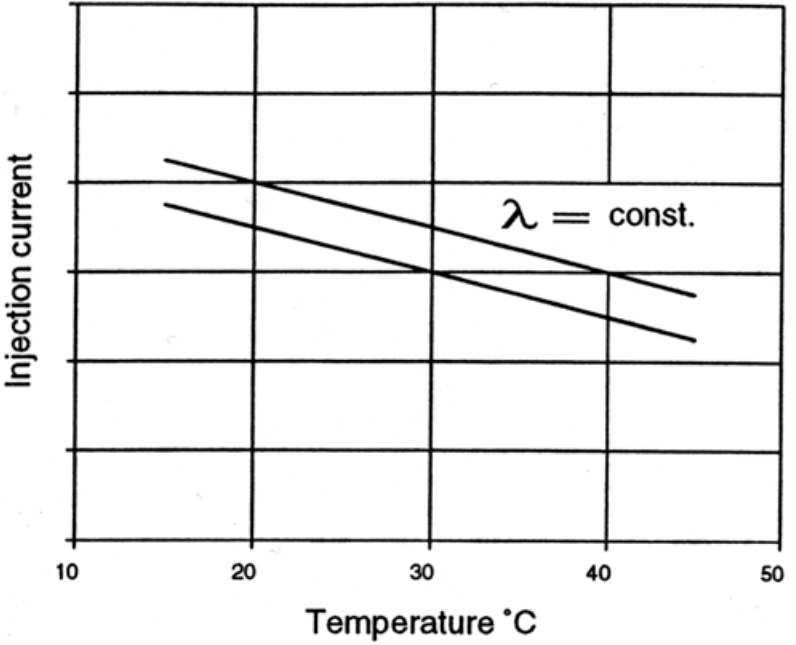
\includegraphics[width=\textwidth]{stromT.png}
		\caption{Diodenstrom (\tilt{injection current}) über der Temperatur (\tilt{Temperature}) für konstante Wellenlängen $\lambda$}\label{img:stromt}
	\end{subfigure}
	\hspace{0.5cm}
	\begin{subfigure}[htbp]{0.45\textwidth}
		\vspace{-0.9cm}
		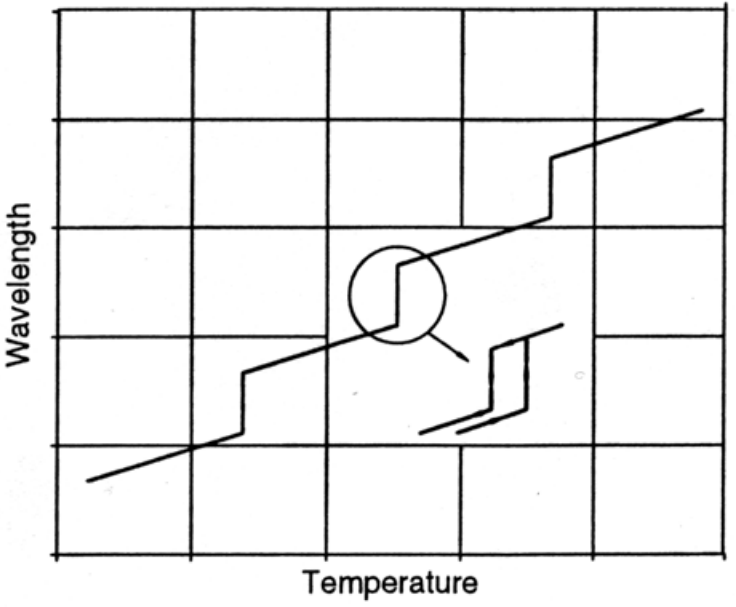
\includegraphics[width=\textwidth]{lambdaT.png}
		\caption{Wellenlänge (\tilt{Wavelength}) des Diodenlasers über Temperatur (\tilt{Temperature})}\label{img:lambdat}
	\end{subfigure}
	\caption{Charakteristische Geraden einer Laser-Diode}
	\label{img:diodechar}
\end{figure}
\subsection{Spektroskopie}
Die Spektroskopie ist eine grundlegende Methode zur quantitativen und qualitativen Untersuchung des Energiespektrums einer Probe in Hinblick auf ihre Wechselwirkung mit einem Strahlungsfeld. Dabei trägt man eine spektrale Größe, wie z.Bsp. die Intensität, gegen eine, von der Energie abhängige Skala auf, was in der Regel die Frequenz oder Wellenlänge ist. Bei der Röntgenspektroskopie trägt man sogar gegen einen Winkel auf (nach \tilt{Bragg}, 1912). Es kann sowohl die Emission und somit Fluoreszenz, als auch die spezifische Absorption im Fokus stehen. Meist wird durch die charakteristische Aufnahme/Abgabe von Energie unter einem einfallenden Strahlungsfeld genutzt, um Rückschlüsse auf die atomare bzw. molekulare Struktur zu ziehen. Die auftretenden Peaks im Spektrum heißen Spektrallinien und sind einzigartig für jede Probe. Sie lassen wegen ihren unterschiedlichen Höhen, unter quantenmechanischer Betrachtung, auch Rückschlüsse auf die Übergangswahrscheinlichkeiten zwischen Energiniveaus zu. In unserem Fall geht es um die Untersuchung eines Neon-Plasmas und somit der Elektronenschale ionisierter Zustände des Edelgases.
\subsection{Fabry-Pérot-Interferometer}
Bei Interferometrie macht man sich, die durch Superposition von Wellen gleicher Frequenzen und verschiedener Phasenbeziehungen erhaltenen, Interferenzbilder zur Nutze. Diese hängen davon ab, welche Form der Kohärenz vorliegt. Schwankt die Phasendifferenz  zwischen $0$ und $2\pi$, so spricht man von inkohärenten Wellen. Ist jedoch für eine Beobachtungszeit $\Delta t$ die Phasendifferenz $\Delta \varphi$ konstant, und gilt $\Delta t>>2\pi/\omega$, so ist das Strahlungsfeld \tilt{zeitlich kohärent}. Liegt im gesamten Raum ein festes $\Delta \varphi$ vor, so spricht man von einem \tilt{räumlich kohärenten} Strahlungsfeld. Das entsprechenden \tilt{Kohörenzvolumen} ist das Produkt aus Kohärenzlänge $c\Delta t$ und der Fläche, welche aus allen Punkten $m$,$n$ mit $|\varphi\ix{m}-\varphi\ix{n}|>\pi$ besteht.
\newpage
Das \tilt{Fabry-Pérot}-Interferometer besteht aus zwei teildurchlässigen, planparallelen Spiegeln, welche den optischen Resonator bilden. Einerseits kann dies durch 2 einzelne, reflektierende Oberflächen mit entspiegelten Rückseiten oder durch einen einzelnen, kubischen Resonatorkörper mit spiegelnden Außenseiten realisiert werden. Letzteres bezeichnet man als \fett{Fabry-Pérot-Etalon}.\\
Eine, unter dem Winkel $\gamma$ zum Lot einfallende Welle der Intensität $I\ix{0}$ wird innerhalb des FPI vielfach reflektiert als auch nach außen transmittiert. Die Interferenz der Strahlung kann nur innerhalb des Kohärenzvolumens beobachtet werden. Hinzu kommt, das die optische Wegdifferenz $\Delta s$ der Teilwellen nicht größer als die Kohärenzlänge sein darf.
\subsection{Zeeman-Effekt}
\subsection{Spektrale Linienbreite}
\section{Durchführung}
\section{Auswertung}
\section{Quellen}
\end{document}